\documentclass[a4paper,10pt,twocolumn,oneside]{article}
\setlength{\columnsep}{10pt}                                                                    %兩欄模式的間距
\setlength{\columnseprule}{0pt}                                                                %兩欄模式間格線粗細

\usepackage{amsthm}								%定義,例題
\usepackage{amssymb}
%\usepackage[margin=2cm]{geometry}
%\usepackage[margin=2cm]{geometry}
\usepackage{fontspec}								%設定字體
\usepackage{color}
\usepackage[x11names]{xcolor}
\usepackage{listings}								%顯示code用的
%\usepackage[Glenn]{fncychap}						%排版,頁面模板
\usepackage{fancyhdr}								%設定頁首頁尾
\usepackage{graphicx}								%Graphic
\usepackage{enumerate}
\usepackage{multicol}
\usepackage{titlesec}
\usepackage{amsmath}
\usepackage{tikz}
\usepackage[CheckSingle, CJKmath]{xeCJK}
\usepackage{savetrees}
\usepackage{array}
\usepackage{xparse}
% \usepackage{CJKulem}

%\usepackage[T1]{fontenc}
\usepackage{amsmath, courier, listings, fancyhdr, graphicx}
\topmargin=0pt
\headsep=5pt
\textheight=780pt
\footskip=0pt
\voffset=-40pt
\textwidth=545pt
\marginparsep=0pt
\marginparwidth=0pt
\marginparpush=0pt
\oddsidemargin=0pt
\evensidemargin=0pt
\hoffset=-42pt

\titlespacing\section{0pt}{-2pt plus 0pt minus 2pt}{-1pt plus 0pt minus 2pt}
\titlespacing\subsection{0pt}{-2pt plus 0pt minus 2pt}{-1pt plus 0pt minus 2pt}
\titlespacing\subsubsection{0pt}{-2pt plus 0pt minus 2pt}{-1pt plus 0pt minus 2pt}


%\renewcommand\listfigurename{圖目錄}
%\renewcommand\listtablename{表目錄} 

%%%%%%%%%%%%%%%%%%%%%%%%%%%%%

\setmainfont [				%主要字型
    Path = .fonts/ttf/,
    UprightFont = *-R,
    BoldFont = *-B,
    ItalicFont = *-RI
  ] {Ubuntu}

\setmonofont [        
    Path = .fonts/ttf/,
    UprightFont = *-R
  ] {UbuntuMono}
% \setmainfont{.fonts/ttf/Ubuntu-R.ttf}				%主要字型
% \setmonofont{.fonts/ttf/UbuntuMono-R.ttf}
\XeTeXlinebreaklocale "zh"						%中文自動換行
\XeTeXlinebreakskip = 0pt plus 1pt				%設定段落之間的距離
\setcounter{secnumdepth}{3}						%目錄顯示第三層

%%%%%%%%%%%%%%%%%%%%%%%%%%%%%
\newcommand\digitstyle{\color{DarkOrchid3}}
\makeatletter
\lst@CCPutMacro\lst@ProcessOther {"2D}{\lst@ttfamily{-{}}{-{}}}
\@empty\z@\@empty

\newtoks\BBQube@token
\newcount\BBQube@length
\def\BBQube@ResetToken{\BBQube@token{}\BBQube@length\z@}
\def\BBQube@Append#1{\advance\BBQube@length\@ne
  \BBQube@token=\expandafter{\the\BBQube@token#1}}

\def\BBQube@ProcessChar#1{%
  \ifnum\lst@mode=\lst@Pmode%
    \ifnum 9<1#1%
      \expandafter\BBQube@Append{\begingroup\digitstyle #1 \endgroup}%
    \else%
      \expandafter\BBQube@Append{#1}%
    \fi%
  \else%
    \expandafter\BBQube@Append{#1}%
  \fi%
}
\def\BBQube@ProcessStringInner#1#2\BBQube@nil{%
  \expandafter\BBQube@ProcessChar{#1}%
  \if\relax\detokenize{#2}\relax%
  \else%
    \expandafter\BBQube@ProcessStringInner#2\BBQube@nil%
  \fi%
}

\def\BBQube@ProcessString#1{\expandafter\BBQube@ProcessStringInner#1\BBQube@nil}

\lst@AddToHook{OutputOther}{%
\BBQube@ResetToken%
\expandafter\BBQube@ProcessString{\the\lst@token}%
\lst@token=\expandafter{\the\BBQube@token}%
}
\makeatother
\lstset{											% Code顯示
language=C++,										% the language of the code
basicstyle=\footnotesize\ttfamily, 						% the size of the fonts that are used for the code
%numbers=left,										% where to put the line-numbers
numberstyle=\footnotesize,						% the size of the fonts that are used for the line-numbers
stepnumber=1,										% the step between two line-numbers. If it's 1, each line  will be numbered
numbersep=5pt,										% how far the line-numbers are from the code
backgroundcolor=\color{white},					% choose the background color. You must add \usepackage{color}
showspaces=false,									% show spaces adding particular underscores
showstringspaces=false,							% underline spaces within strings
showtabs=false,									% show tabs within strings adding particular underscores
frame=false,											% adds a frame around the code
tabsize=2,											% sets default tabsize to 2 spaces
captionpos=b,										% sets the caption-position to bottom
breaklines=true,									% sets automatic line breaking
breakatwhitespace=false,							% sets if automatic breaks should only happen at whitespace
escapeinside={\%*}{*)},							% if you want to add a comment within your code
morekeywords={constexpr},									% if you want to add more keywords to the set
keywordstyle=\bfseries\color{Blue1},
commentstyle=\itshape\color{Red4},
stringstyle=\itshape\color{Green4},
}

%%%%%%%%%%%%%%%%%%%%%%%%%%%%%

\ExplSyntaxOn
\NewDocumentCommand{\captureshell}{som}
 {
  \sdaau_captureshell:Ne \l__sdaau_captureshell_out_tl { #3 }
  \IfBooleanT { #1 }
   {% we may need to stringify the result
    \tl_set:Nx \l__sdaau_captureshell_out_tl
     { \tl_to_str:N \l__sdaau_captureshell_out_tl }
   }
  \IfNoValueTF { #2 }
   {
    \tl_use:N \l__sdaau_captureshell_out_tl
   }
   {
    \tl_set_eq:NN #2 \l__sdaau_captureshell_out_tl
   }
 }

\tl_new:N \l__sdaau_captureshell_out_tl

\cs_new_protected:Nn \sdaau_captureshell:Nn
 {
  \sys_get_shell:nnN { #2 } { } #1
  \tl_trim_spaces:N #1 % remove leading and trailing spaces
 }
\cs_generate_variant:Nn \sdaau_captureshell:Nn { Ne }
\ExplSyntaxOff

\begin{document}
\pagestyle{fancy}
\fancyfoot{}
%\fancyfoot[R]{\includegraphics[width=20pt]{ironwood.jpg}}
\fancyhead[L]{National Tsing Hua University Kenapsack}
\fancyhead[R]{\thepage}
\renewcommand{\headrulewidth}{0.4pt}
\renewcommand{\contentsname}{Contents} 
\newcommand{\inputcode}[2]{
    \subsection[#1]{#1}
    \lstinputlisting{#2}
}

\textbf{
\scriptsize
\tableofcontents
}
%%%%%%%%%%%%%%%%%%%%%%%%%%%%%

% \newpage

\footnotesize

\section{Basic}
\subsection{.vimrc}
\lstinputlisting{1_Basic/.vimrc}
\inputcode{Default Bear}{1_Basic/default_bear.cpp}
\inputcode{Default Ken}{1_Basic/DEFAULT_KEN.cpp}
\inputcode{IO Optimize}{1_Basic/IO_Optimize.cpp}
\inputcode{PBDS}{1_Basic/PBDS.cpp}
\inputcode{Random}{1_Basic/Random.cpp}
\inputcode{Python}{1_Basic/Python.py}
\inputcode{Set Comperator}{1_Basic/set_comperator.cpp}

\section{Graph}
\inputcode{2 SAT}{2_Graph/2_SAT.cpp}
\inputcode{Bellman Ford}{2_Graph/Bellman_Ford.cpp}
\inputcode{Biconnected Component}{2_Graph/Biconnected_Component.cpp}
\inputcode{Bridge}{2_Graph/Bridge.cpp}
\inputcode{Bridge Connected Component}{2_Graph/Bridge_Connected_Component.cpp}
\inputcode{Centroid Decomposition}{2_Graph/Centroid_Decomposition.cpp}
\inputcode{Close Vertices}{2_Graph/Close_Vertices.cpp}
\inputcode{Disjoint Set}{2_Graph/Disjoint_Set.cpp}
\inputcode{Heavy Light Decomposition}{2_Graph/Heavy_Light_Decomposition.cpp}
\inputcode{KSP}{2_Graph/KSP.cpp}
\inputcode{LCA}{2_Graph/LCA.cpp}
\inputcode{Maximum Clique}{2_Graph/Maximum_Clique.cpp}
\inputcode{SCC Kosaraju}{2_Graph/SCC_Kosaraju.cpp}
\inputcode{SCC Tarjan}{2_Graph/SCC_Tarjan.cpp}
\inputcode{Tree Centroid}{2_Graph/Tree_Centroid.cpp}
\inputcode{Virtual Tree}{2_Graph/Virtual_Tree.cpp}


\section{Data Structure}
\inputcode{2D BIT          }{3_Data_Structure/2D_BIT.cpp}
\inputcode{2D Segment Tree }{3_Data_Structure/2D_Segment_Tree.cpp}
\inputcode{BIT             }{3_Data_Structure/BIT.cpp}
\inputcode{chtholly tree   }{3_Data_Structure/chtholly_tree.cpp}
\inputcode{LiChaoST        }{3_Data_Structure/LiChaoST.cpp}
\inputcode{persistent      }{3_Data_Structure/persistent.cpp}
\inputcode{Sparse Table    }{3_Data_Structure/Sparse_Table.cpp}
\inputcode{Treap           }{3_Data_Structure/Treap.cpp}
\inputcode{ZKW Segment Tree}{3_Data_Structure/ZKW_Segment_Tree.cpp}


\section{Flow}
\inputcode{Bipartite Matching           }{4_Flow/Bipartite_Matching.cpp                                               }
\inputcode{Dinic                        }{4_Flow/Dinic.cpp                                                            }
\inputcode{KM                           }{4_Flow/KM.cpp                                                               }
\inputcode{Maximum Simple Graph Matching}{4_Flow/Maximum_Simple_Graph_Matching.cpp                                    }
\inputcode{MCMF                         }{4_Flow/MCMF.cpp                                                             }


\section{Geometry}
\inputcode{Basic 2D                 }{5_Geometry/Basic_2D.cpp                                                         }
\inputcode{Convex Hull              }{5_Geometry/Convex_Hull.cpp                                                      }
\inputcode{Dynamic Convex Hull      }{5_Geometry/Dynamic_Convex_Hull.cpp                                              }
\inputcode{Segmentation Intersection}{5_Geometry/Segmentation_Intersection.cpp                                        }
% \subsection{Theorem}
% \begin{itemize}[leftmargin=*]
\setlength\itemsep{0.2em}
\item Pick's Theorem:\\
if a polygon has vertices with integer coordinates (lattice points), then the area is $i+\frac{1}{2}p−1$ where $i$ is the number of lattice points inside the polygon and $p$ is the number of lattice points on the perimeter of the polygon. i.e.
$$area(P)=i+\frac{1}{2}p-1$$

\end{itemize}


\section{Math}
\inputcode{Big Int          }{6_Math/Big_Int.cpp                                                          }
\inputcode{Chinese Remainder}{6_Math/Chinese_Remainder.cpp                                                }
\inputcode{Extgcd           }{6_Math/Extgcd.cpp                                                           }
\inputcode{Karatsuba        }{6_Math/Karatsuba.cpp                                                        }
\inputcode{Linear Sieve     }{6_Math/Linear_Sieve.cpp                                                     }
\inputcode{Matrix           }{6_Math/Matrix.cpp                                                           }
\inputcode{Miller Rabin     }{6_Math/Miller_Rabin.cpp                                                     }
\inputcode{NTT              }{6_Math/NTT.cpp                                                              }
\inputcode{Pollard Rho      }{6_Math/Pollard_Rho.cpp                                                      }
\inputcode{Primes           }{6_Math/Primes.cpp                                                           }


\section{String}
%\subsection{AC}
%\lstinputlisting{7_String/AC.cpp}
%\subsection{Hash}
%\lstinputlisting{7_String/Hash.cpp}
%
%\subsection{KMP}
%\lstinputlisting{7_String/KMP.cpp}
%
%\subsection{Manacher}
%\lstinputlisting{7_String/Manacher.cpp}
%
%\subsection{SA}
%\lstinputlisting{7_String/SA.cpp}
%
%%\subsection{SA2}
%%\lstinputlisting{7_String/SA2.cpp}
%
%\subsection{SAIS}
%\lstinputlisting{7_String/SAIS.cpp}
%
%\subsection{Z}
%\lstinputlisting{7_String/Z.cpp}
%
%\section{Others}
%\subsection{Mo}
%\lstinputlisting{8_Others/Mo.cpp}
%
%\subsection{Partial Ordering}
%\lstinputlisting{8_Others/Partial_Ordering.cpp}

\newpage
\foreach \p in {1,2,3} { % 生成三頁
    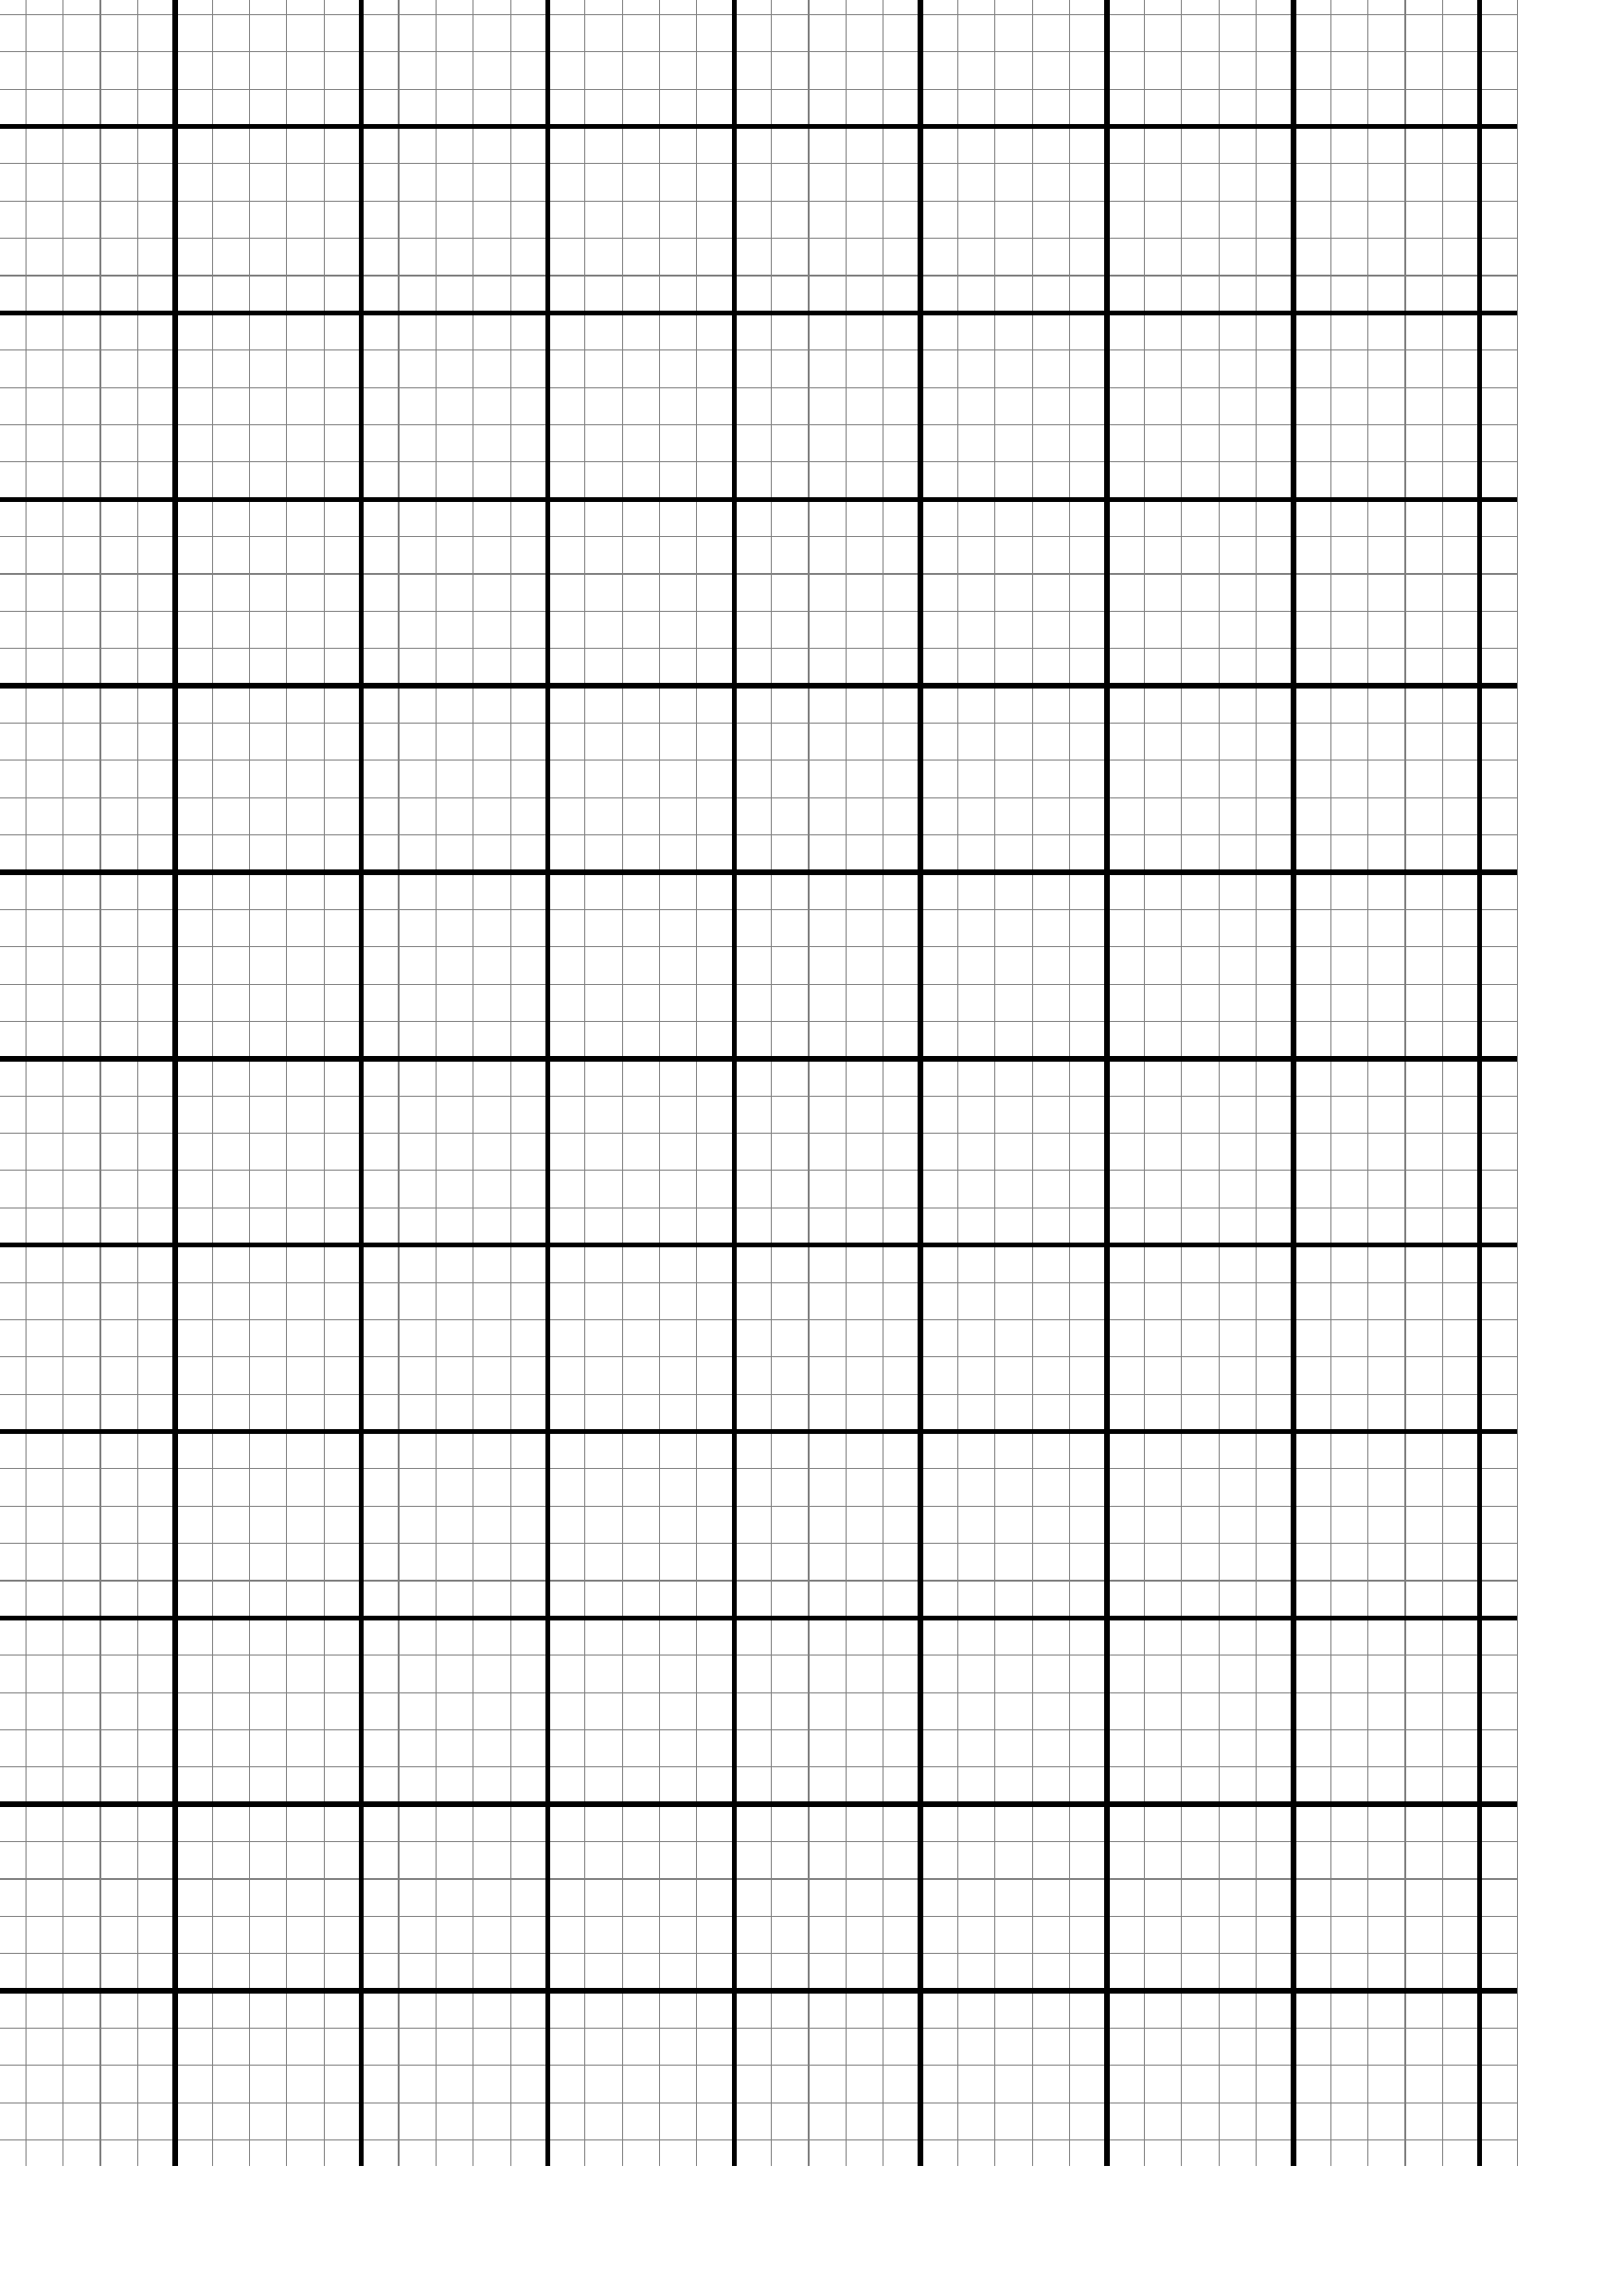
\begin{tikzpicture}[scale=1]
        % 設定 A4 紙張大小並居中
        \draw[step=0.5cm, gray] (-10.5, -14.85) grid (10.5, 14.85); % 設定細線網格
        \draw[step=2.5cm, line width=0.7mm] (-10.5, -14.85) grid (10.5, 14.85); % 設定粗線網格
    \end{tikzpicture}
    \newpage % 生成新頁面
}

\end{document}
